\begin{frame}
\frametitle{Transmission without specific component}
\begin{block}{Our target (remind)}
Use electromagnetic emanations to create a covert channel and exfiltrate data
\end{block}
\begin{alertblock}{Problems}
\begin{itemize}
\item Computer's electromagnetic emanations $\rightarrow$ low amplitude
\item Amplitude increase $\Rightarrow$ circuit tension increase
\end{itemize}
\end{alertblock}
\end{frame}

\begin{frame}
\frametitle{Problem bypass : Multi-channel memory architectures}

\begin{columns}[c] % align columns
\begin{column}{.28\textwidth}
\centering 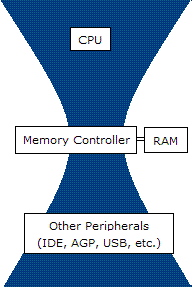
\includegraphics[scale=.3]{images/goulot.png}
\end{column}%
\hfill%
\begin{column}{.68\textwidth}
\begin{block}{Memory access}
\begin{itemize}
\item Memory controller $\rightarrow$ bottleneck
\item Intel/AMD $\rightarrow$ Multi-channel memory architectures
\item Increase data bus size :
\begin{itemize}
\item Double channel $\Rightarrow$ 128 bits
\item Triple channel $\Rightarrow$ 192 bits
\item Quadruple channel $\Rightarrow$ 256 bits
\end{itemize}
\end{itemize}
\end{block}
\end{column}%
\end{columns}

\end{frame}

\begin{frame}
\frametitle{Problem bypass : Multi-channel memory architectures}

\begin{columns}[c] % align columns
\begin{column}{.33\textwidth}
\centering 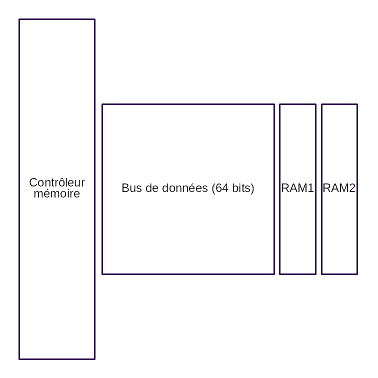
\includegraphics[scale=.4]{images/mono-canal.png}
\end{column}%
%\hfill%
\begin{column}{.01\textwidth}
$\longrightarrow$
\end{column}
\begin{column}{.28\textwidth}
\centering 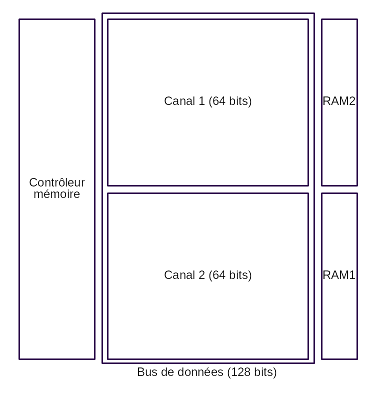
\includegraphics[scale=.4]{images/multi-canal.png}
\end{column}%
\end{columns}

\begin{block}{Consequence using Multi-channel memory}
\begin{itemize}
\item More electrons in movement at the same time
\item Significant electromagnetic emanations created
\item $\Rightarrow$ Emanations could be used to create covert channel
\end{itemize}
\end{block}

\end{frame}

\begin{frame}
\frametitle{Problem bypass : Multi-channel memory architectures}

\begin{columns}[c] % align columns
\begin{column}{.28\textwidth}
\centering 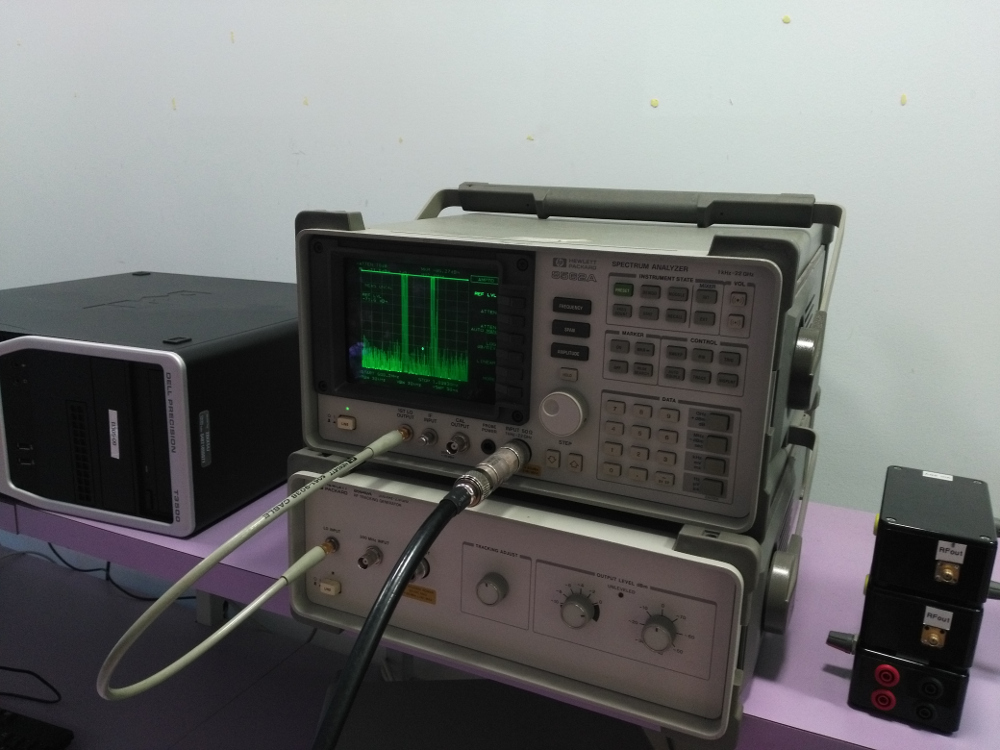
\includegraphics[scale=.13]{images/spectrum.jpg}
\end{column}%
\hfill%
\begin{column}{.5\textwidth}
\begin{block}{Application}
\begin{itemize}
\item Be sure to bypass CPU optimizations
\item Use of \texttt{MOVNTDQ} instruction on \texttt{xmm} registers
\item Emanations highlight :
\begin{itemize}
\item Find emission frequency : spectrum analizer
\item Watch signal : USRP/RTL-SDR + URH
\end{itemize}
\end{itemize}
\end{block}
\end{column}%
\end{columns}

\end{frame}



\begin{frame}
\frametitle{Problem bypass : Multi-channel memory architectures}

\centering 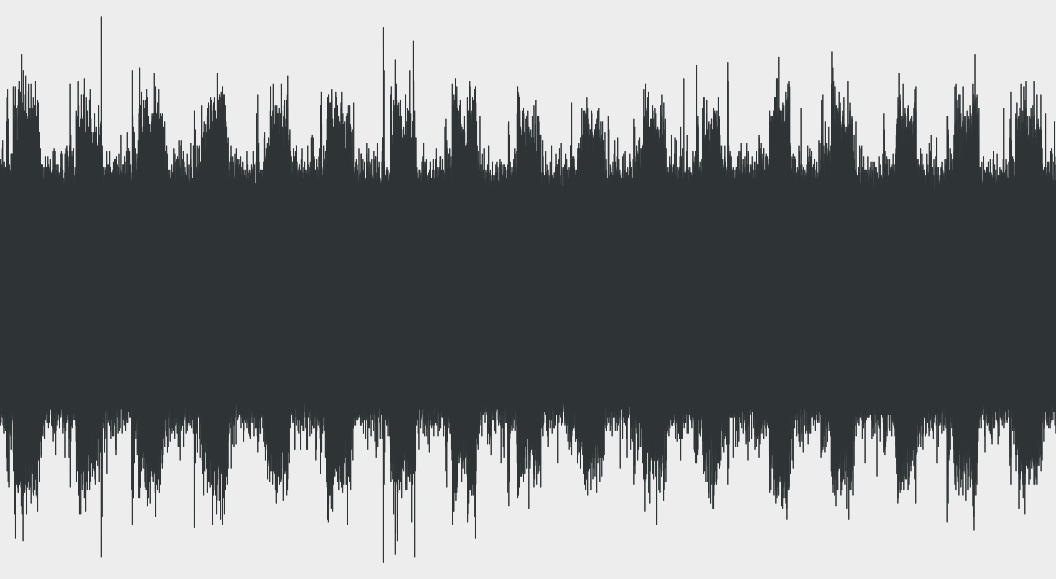
\includegraphics[scale=.2]{images/signal.png}

\begin{block}{Modulation}
\begin{itemize}
\item Modulation = information coding process
\item Binary Amplitude-Shift Keying (B-ASK) modulation :
\begin{itemize}
\item bit 0 $\leftrightarrow$ normal emission level
\item bit 1 $\leftrightarrow$ average emission level when multi-channel memory is used
\end{itemize}
\end{itemize}
\end{block}

\end{frame}